\section{Three-dimensional simulations}
The 3D disc has radial size 
$[r_\mathrm{min},r_\mathrm{max}]=[0.4,10]R_0$ and vertical extent
$n_H=2$ scale-heights. The resolution is $N_r\times N_\theta\times
N_\phi=256\times32\times256$. Because of the much reduced resolution
compared to 2D, we use a smooth perturbation by setting
$\delta = 10^{-3}$ and $M=1$. This corresponds to a single $m=1$
spiral in the dead zone, which was found to dominate the 2D
simulation. 

Our 3D discs are initialised in approximate equilibrium only, so we
first evolve the disc without perturbations using  
$(\lmax,\mmax)=(32,0)$ up to $t=10P_0$, during which 
meridional velocities are damped out. We then restart the simulation
with the above perturbation and $(\lmax,\mmax)=(32,32)$. 

Snapshots at the end of the simulations are shown in
Fig. \ref{3d_prelim} for both ZEUS-MP and PLUTO. We again find the dead zone eventually
dominated by an $m=1$ spiral. A Cartesian visualisation of the
midplane density perturbation associated with the $m=1$ mode is shown in Fig. \ref{pluto_cart}.
The two codes give qualitatively similar results, but a longer PLUTO simulation was
needed to achieve similar mode amplitudes than ZEUS-MP. 
The amplitude of the spiral is smaller than the 2D case above,
possibily due to lower resolution and/or 3D self-gravity being weaker
than that in 2D.  

\begin{figure}
  \begin{center}
    \subfigure[ZEUS-MP]{
      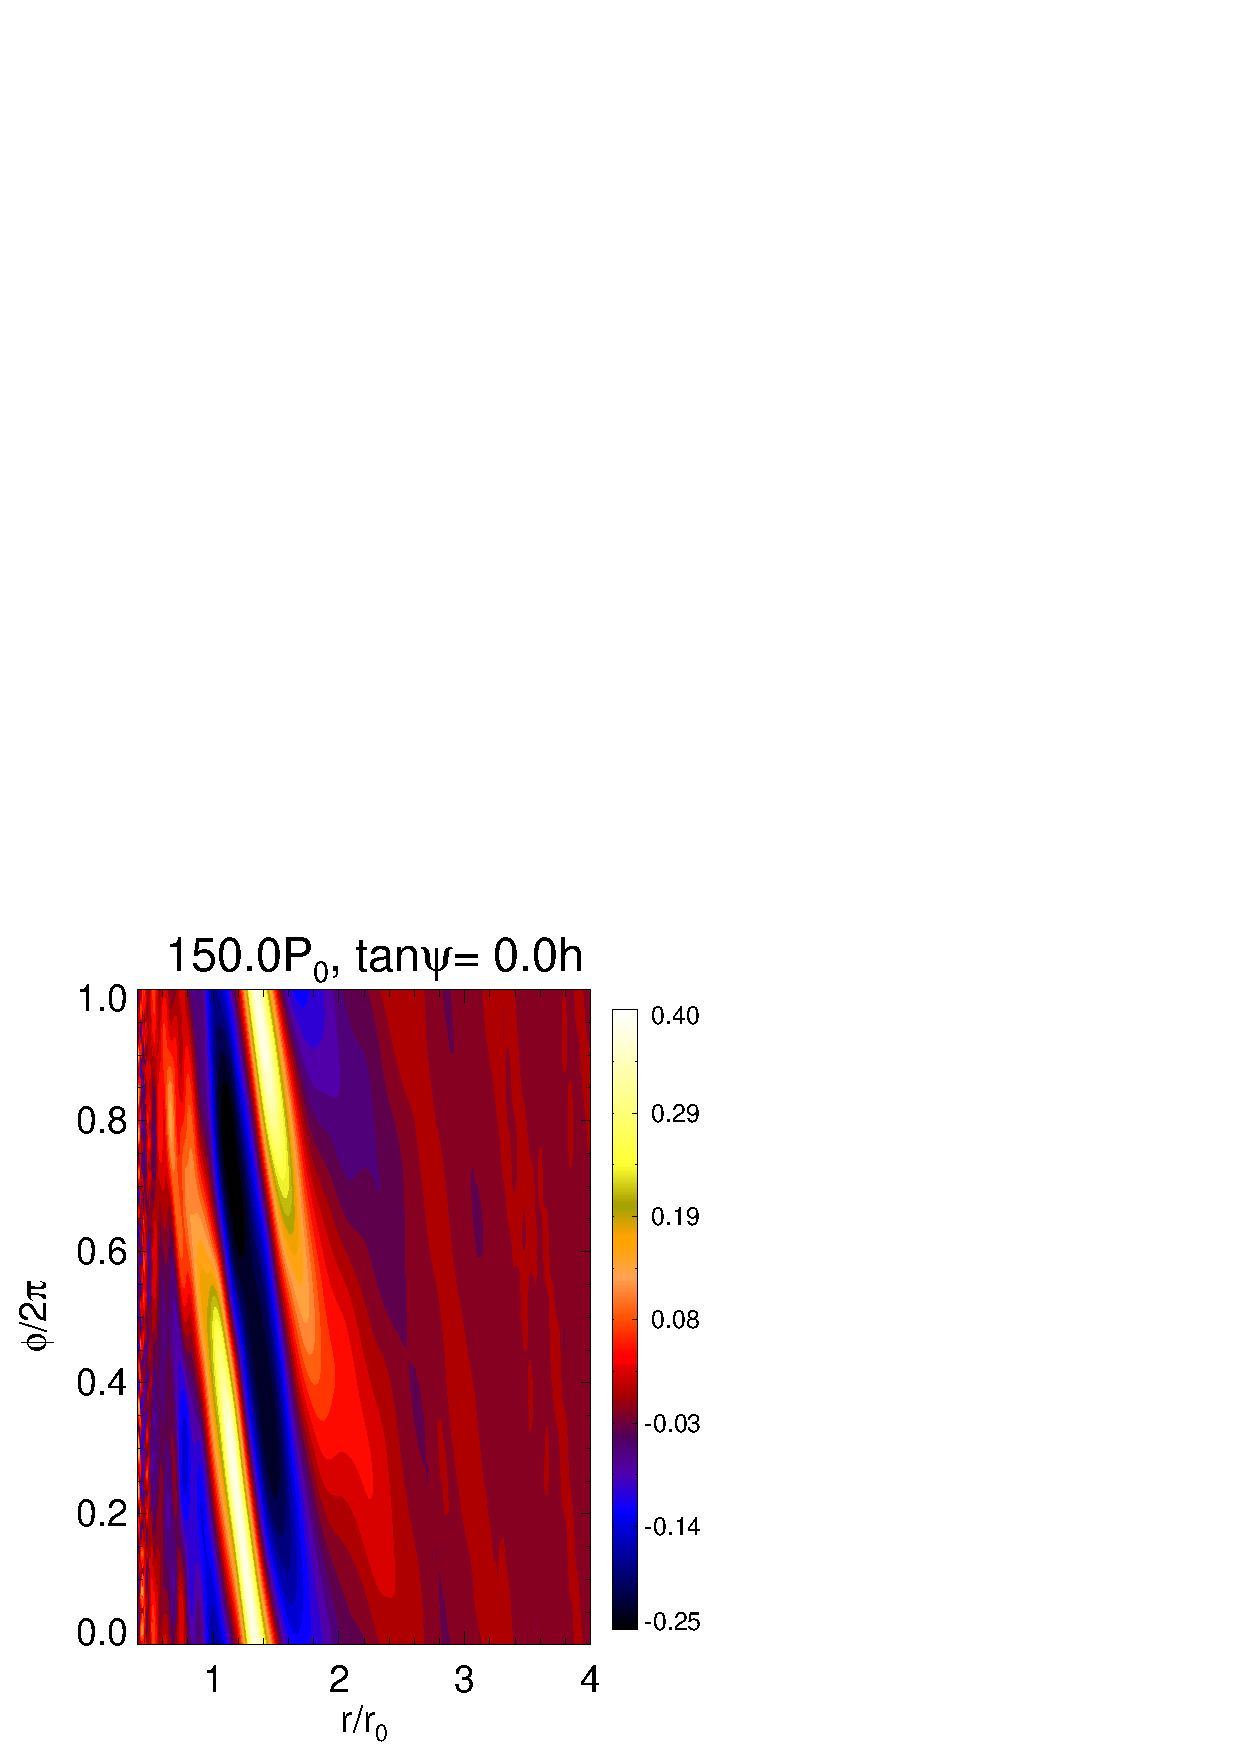
\includegraphics[scale=0.33]{figures/polarxy_dens015_zeus}
    }
    \subfigure[PLUTO]{
      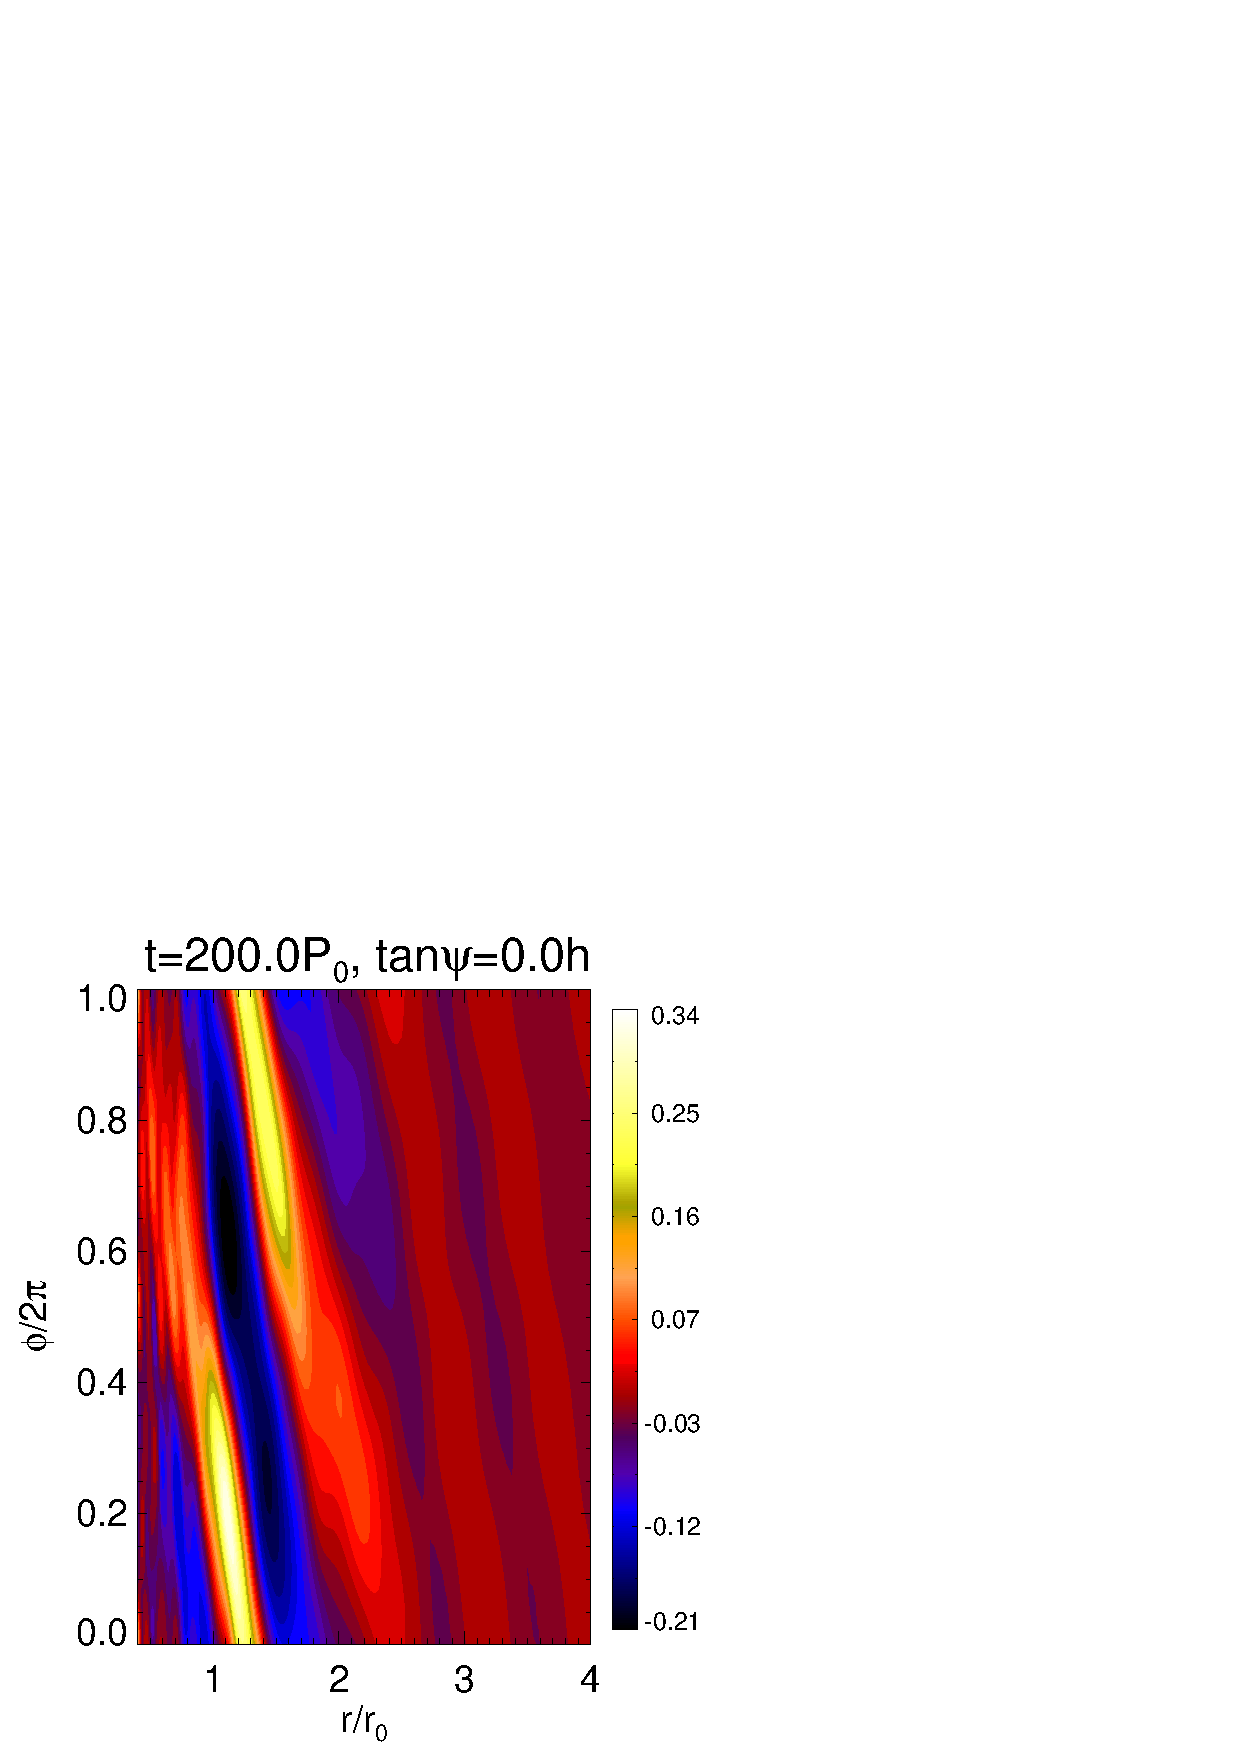
\includegraphics[scale=0.33]{figures/pdisk_020}
    }
  \end{center}
  \caption{Preliminary 3D simulations using the (a) ZEUS-MP and (b)
    PLUTO. The non-axisymmetric midplane density at the end of the run
    is shown. Here $\psi \equiv \pi/2 - \theta$ is the angular height
    from the midplane.\label{3d_prelim}}   
\end{figure}

\begin{figure}
  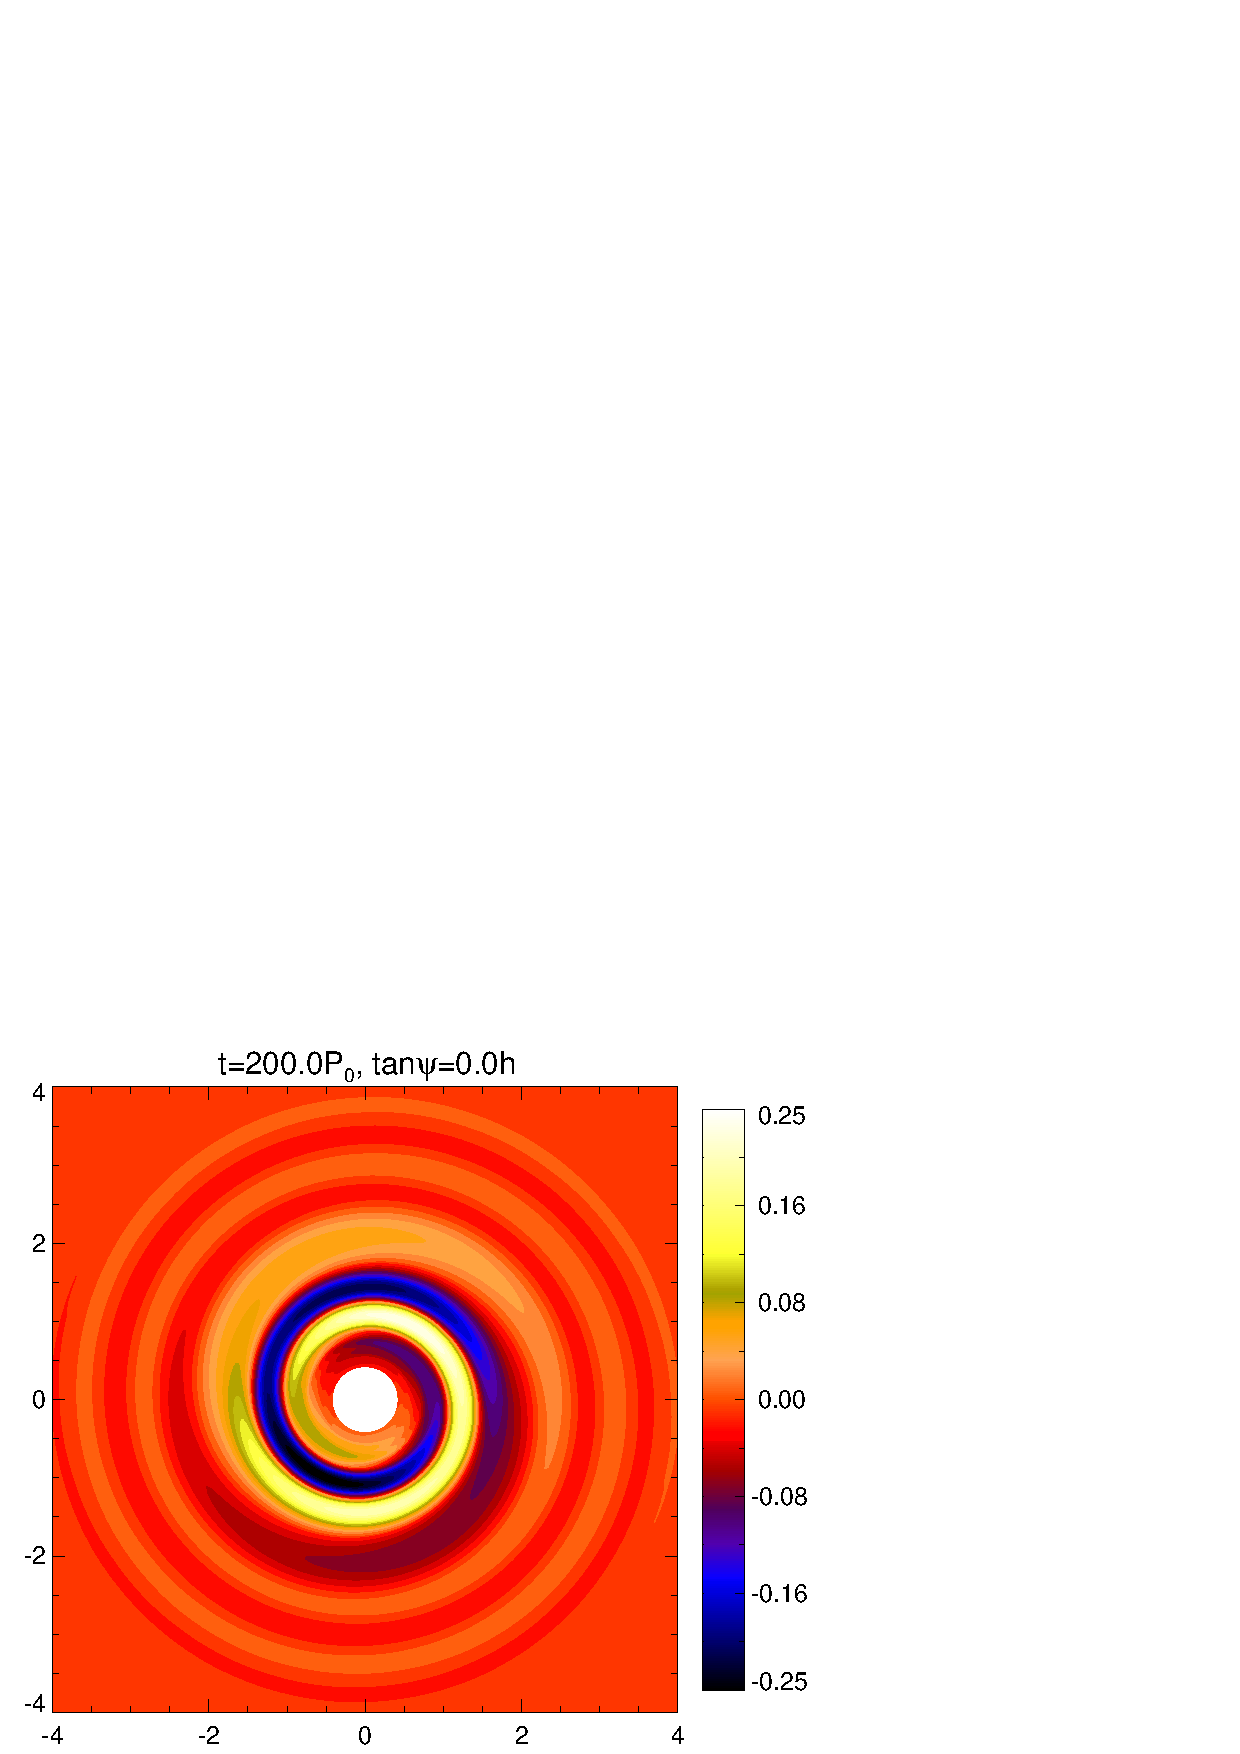
\includegraphics[width=\linewidth]{figures/pdiskxy_020_m1}
  \caption{Cartesian visualisation the $m=1$ midplane density in the PLUTO
    simulation shown in Fig. \ref{3d_prelim}.\label{pluto_cart}}   
\end{figure} 

%\subsection{Angular momentum evolution}


Fig. \ref{3d_angmom} shows the angular momentum evolution in the 3D
runs. ZEUS-MP does not conserve angular momentum very well, but
the variation $|\Delta J/J|< O(10^{-5})$ is not significant compared
to the individual components $|\Delta J_{0,1}/J|\sim 
6\times10^{-5}$. The PLUTO run reaches similar values of
$|J_{0,1}|$, but achieves better conervation, with $|\Delta
J/J|=O(10^{-8})$. 

%Note that FARGO does not explicitly conserve angular
%momentum. In addition, there may be an angular momentum flux due to
%self-gravity across disc boundaries since our domain size is finite. 
%Fig. \ref{prelim_angmom} shows the angular momentum evolution in
%the 3D runs. 

\begin{figure}
%scale=0.41
  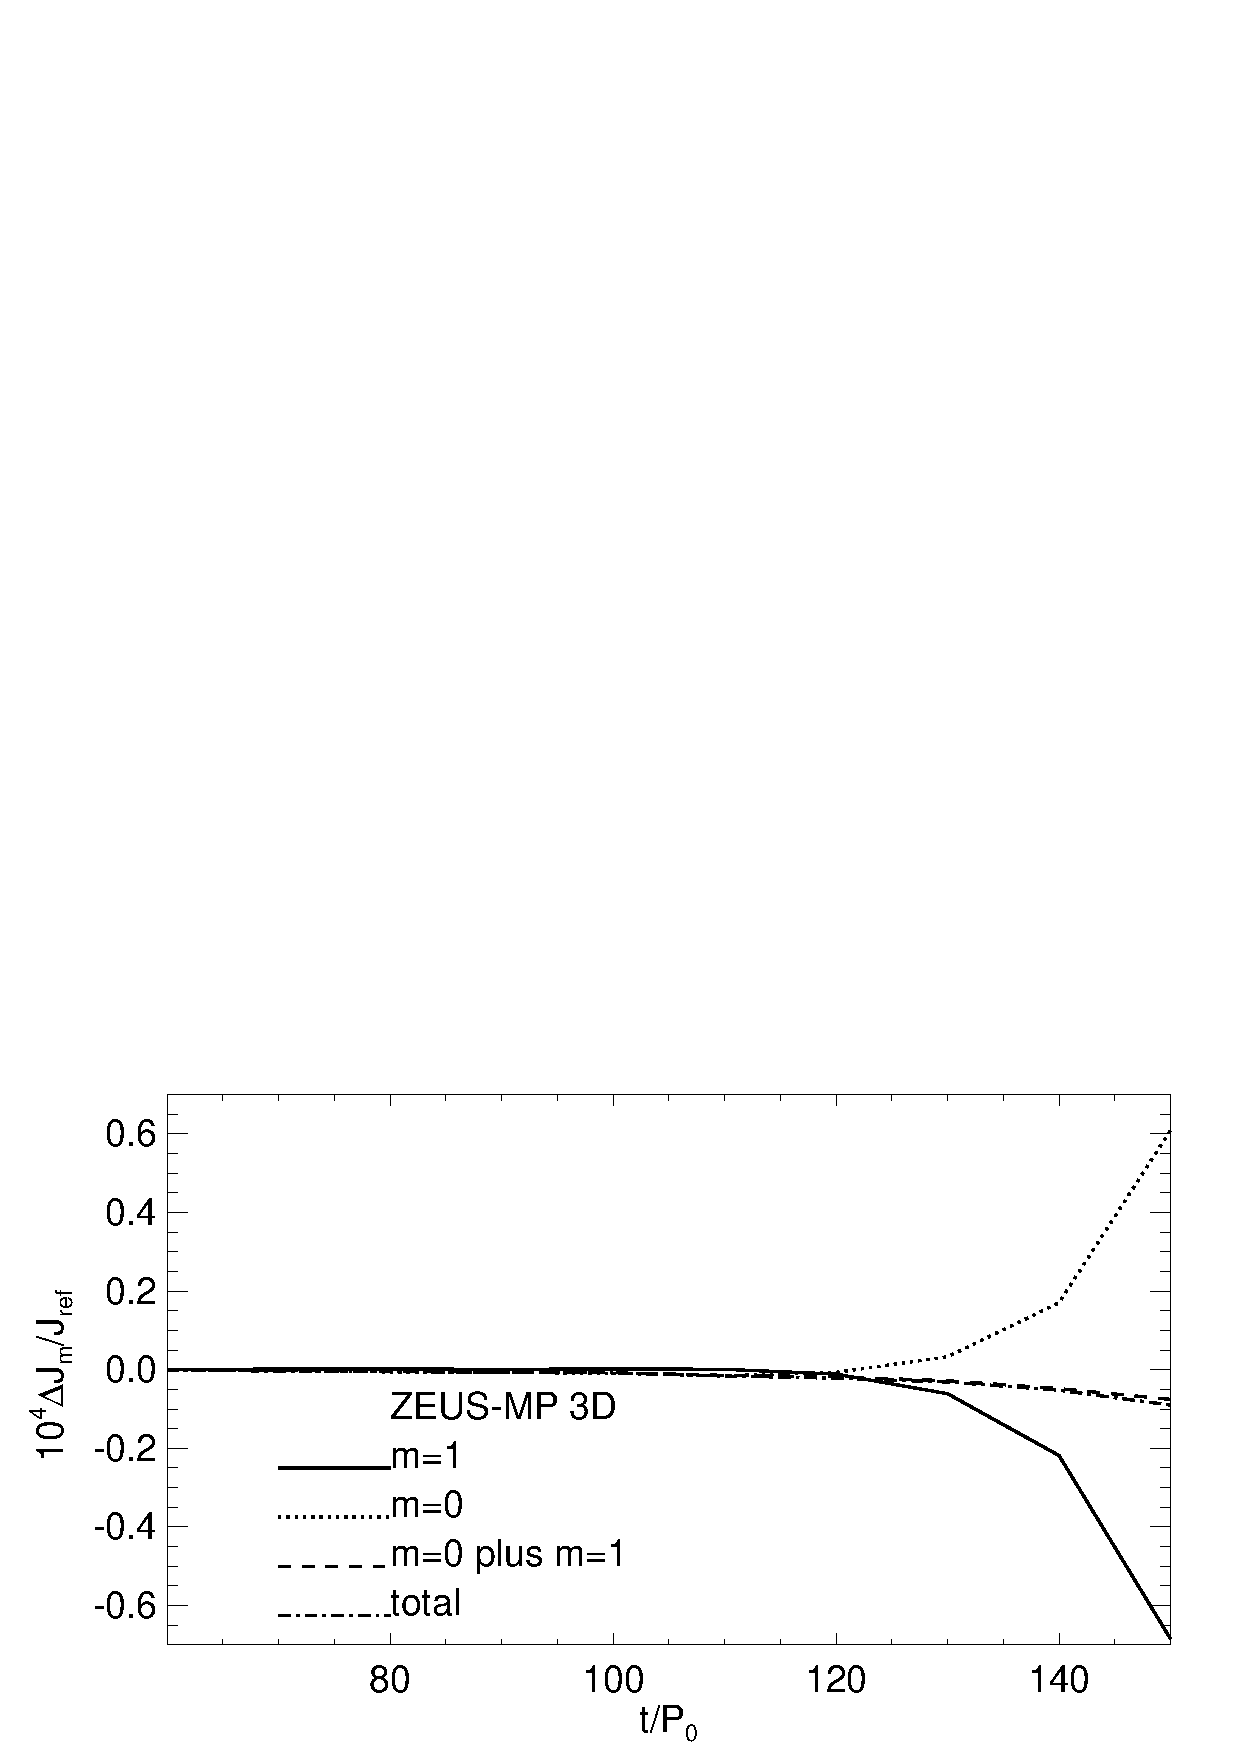
\includegraphics[scale=.41,clip=true,trim=0cm 1cm 0cm 0cm]{figures/nonaxi_evol_ang_zeus}
  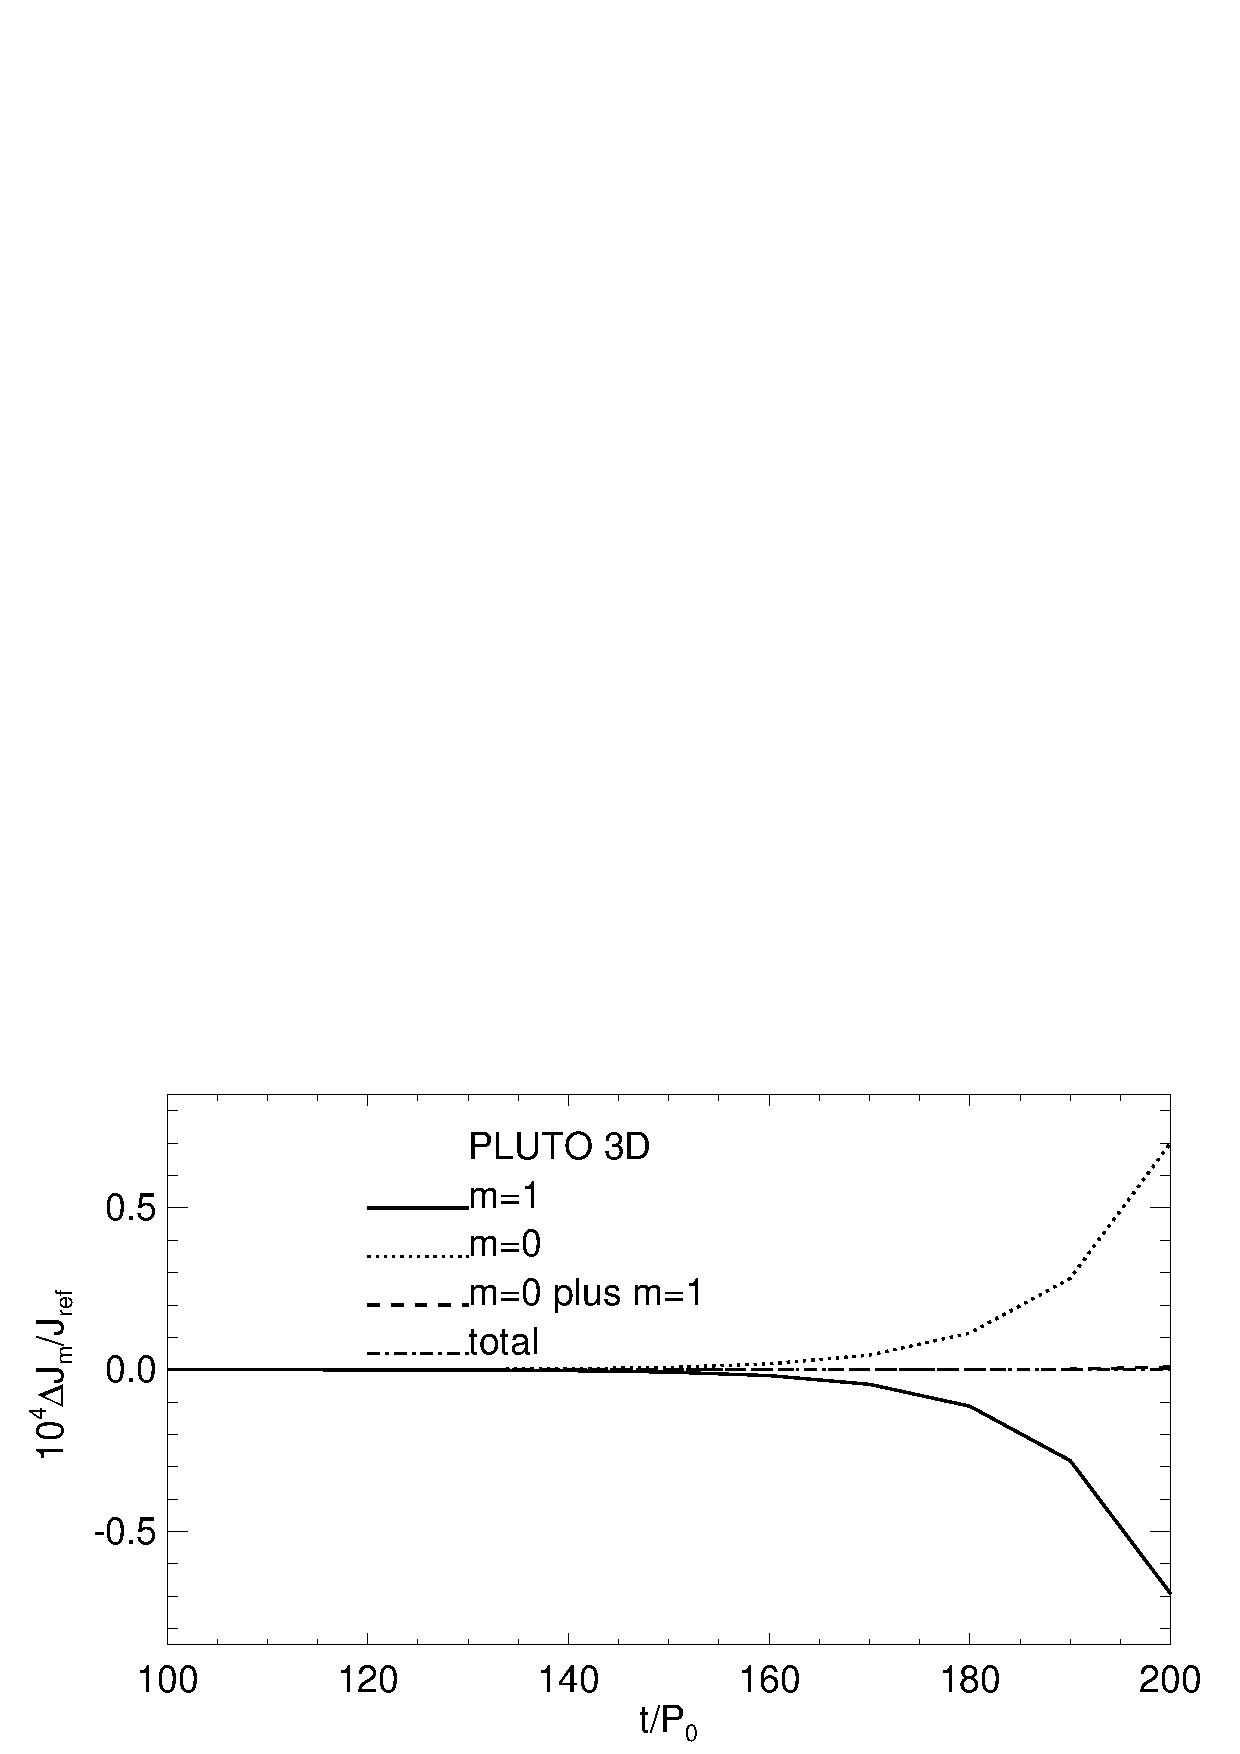
\includegraphics[scale=.41]{figures/nonaxi_evol_ang_pluto}
  \caption{Evolution of angular momentum components in the fiducial 3D 
    simulations. The perturbation
    relative to $t=100P_0$ is shown in units of the
    initial total angular momentum $J_\mathrm{ref}$.\label{3d_angmom}} 
\end{figure}   

% \section{One-arm spirals in structured discs}
% Here we examine a 2D FARGO simulation in more detail. The setup is the
% same as that in \S\ref{fargo_fiducial}, except we use a resolution of
% $N_R\times N_\phi = 2048\times4096$ and initialise the disc with a
% single $m=1$ perturbation.   

% \subsection{Properties of the $m=1$ dead zone spiral}
% % growth rate, co-rotation radius, pattern speed, propagation diagram 

